\chapter{Qualitative analysis and Bayes error}
\label{chap:qualitative_analysis}

In this final chapter, we extend our evaluation beyond the single primary application ($\pi_T = 0.1$) to perform a comprehensive qualitative analysis. We evaluate the models across a wide range of operating points by sweeping the prior log-odds from $-4$ to $+4$. 

For this analysis, we select the top-performing architectures from our parameter search: the \textbf{Diagonal Covariance GMM (16 components)}, the \textbf{Full Covariance GMM (8 components)}, and the \textbf{Tied Covariance GMM (8 components)}.

\section{Bayes Error plots}

The following figures display the Bayes Error plots for the three selected GMM architectures. The blue curves represent the theoretical Minimum DCF, while the red curves represent the Actual DCF obtained using the raw Log-Likelihood Ratios (LLRs).

\begin{figure}[H]
    \centering
    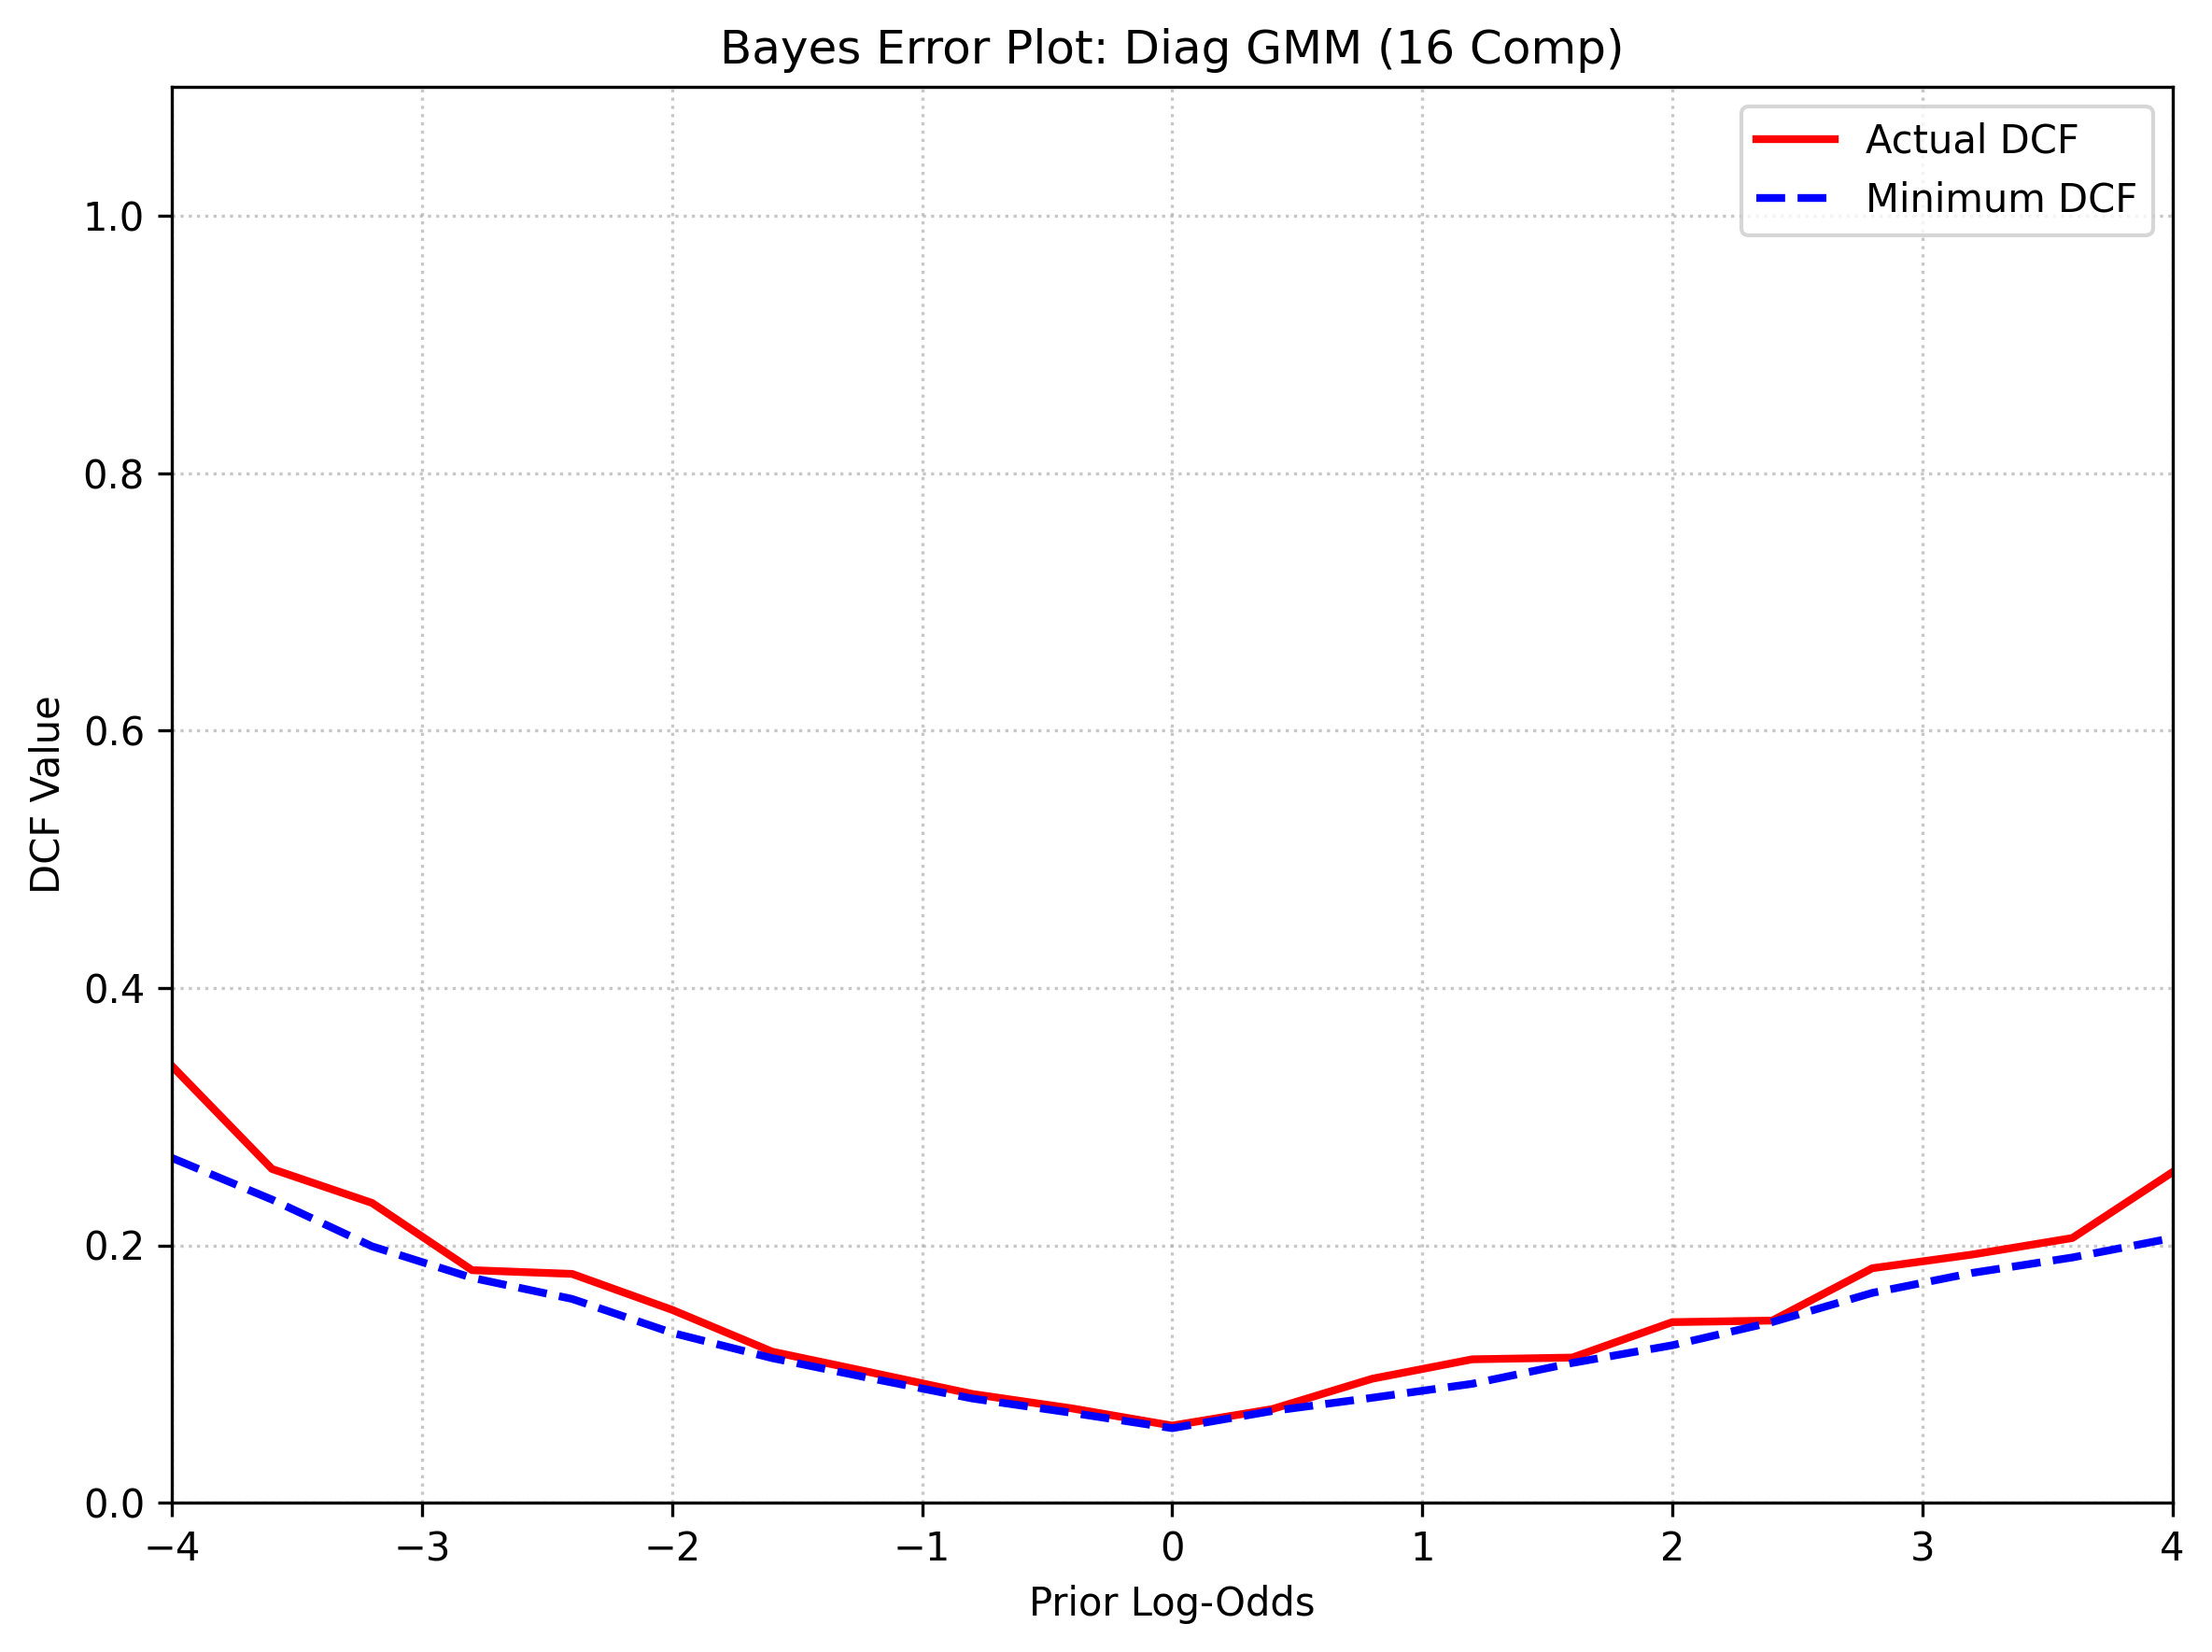
\includegraphics[width=0.75\textwidth]{bayes_error_diag_16comp.png}
    \caption{Bayes Error plot for the Diagonal Covariance GMM with 16 components. The model demonstrates exceptional overall performance and tight calibration.}
    \label{fig:bayes_diag_16}
\end{figure}

\begin{figure}[H]
    \centering
    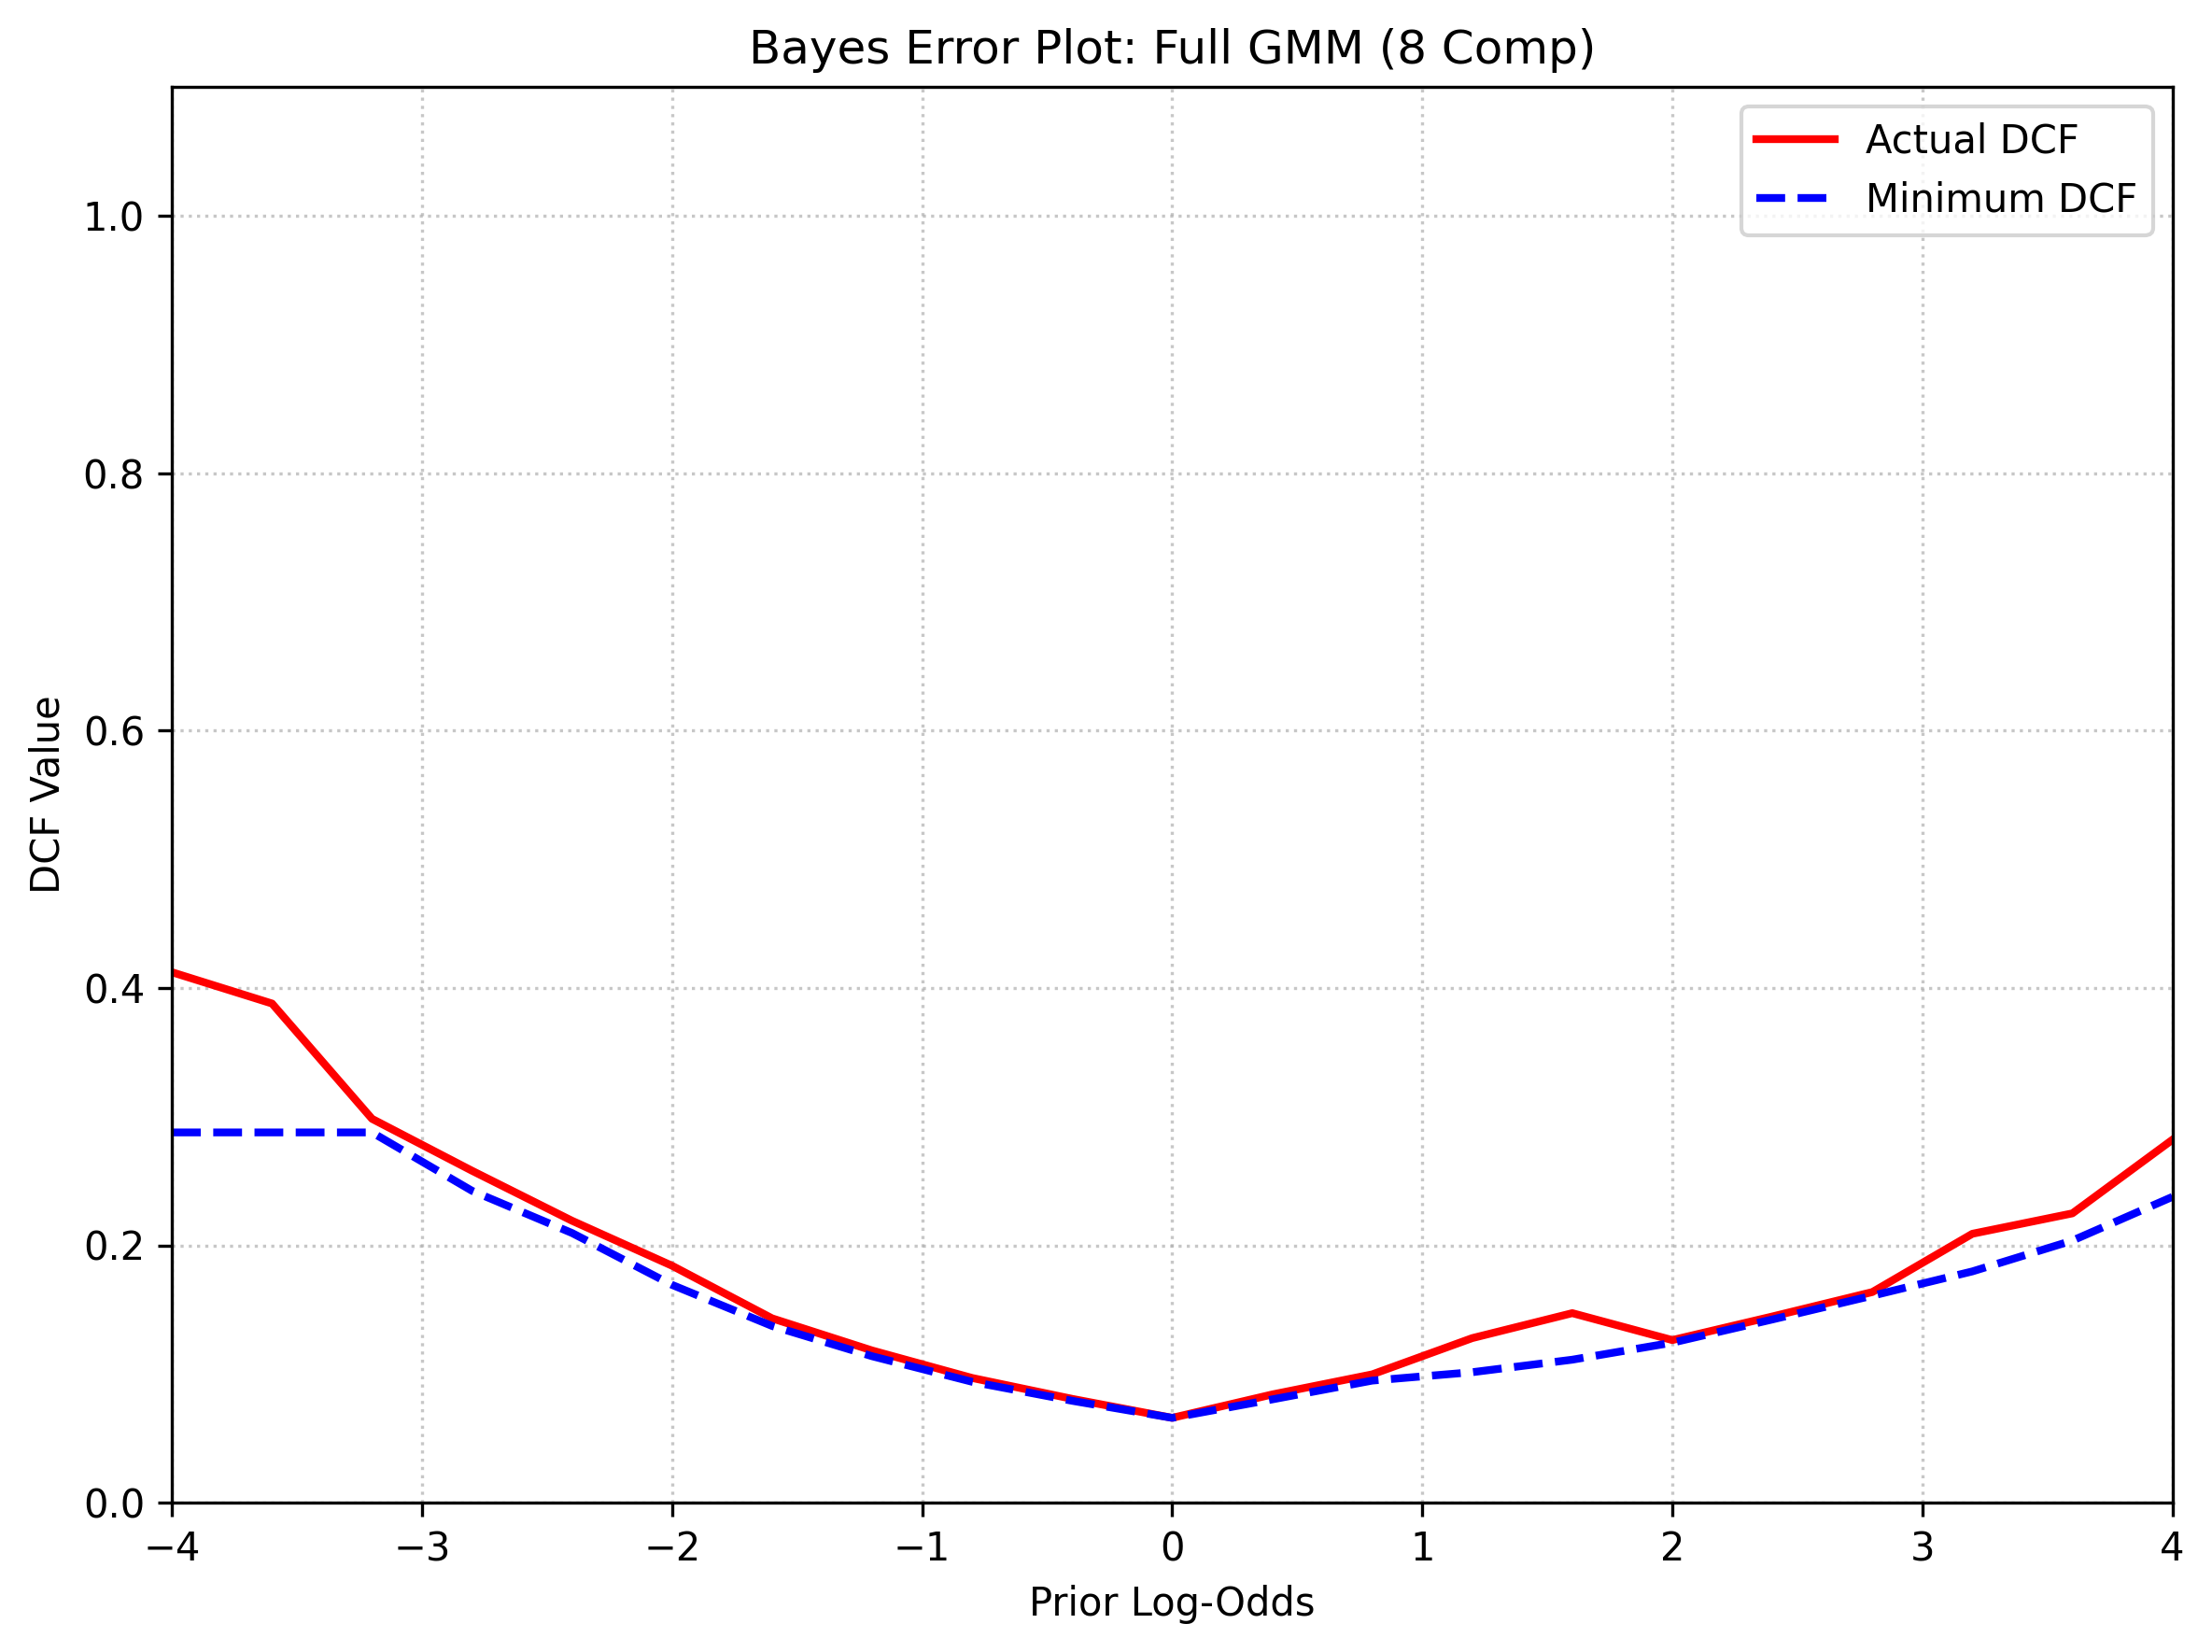
\includegraphics[width=0.75\textwidth]{bayes_error_full_8comp.png}
    \caption{Bayes Error plot for the Full Covariance GMM with 8 components. The calibration remains highly stable across the log-odds spectrum.}
    \label{fig:bayes_full_8}
\end{figure}

\begin{figure}[H]
    \centering
    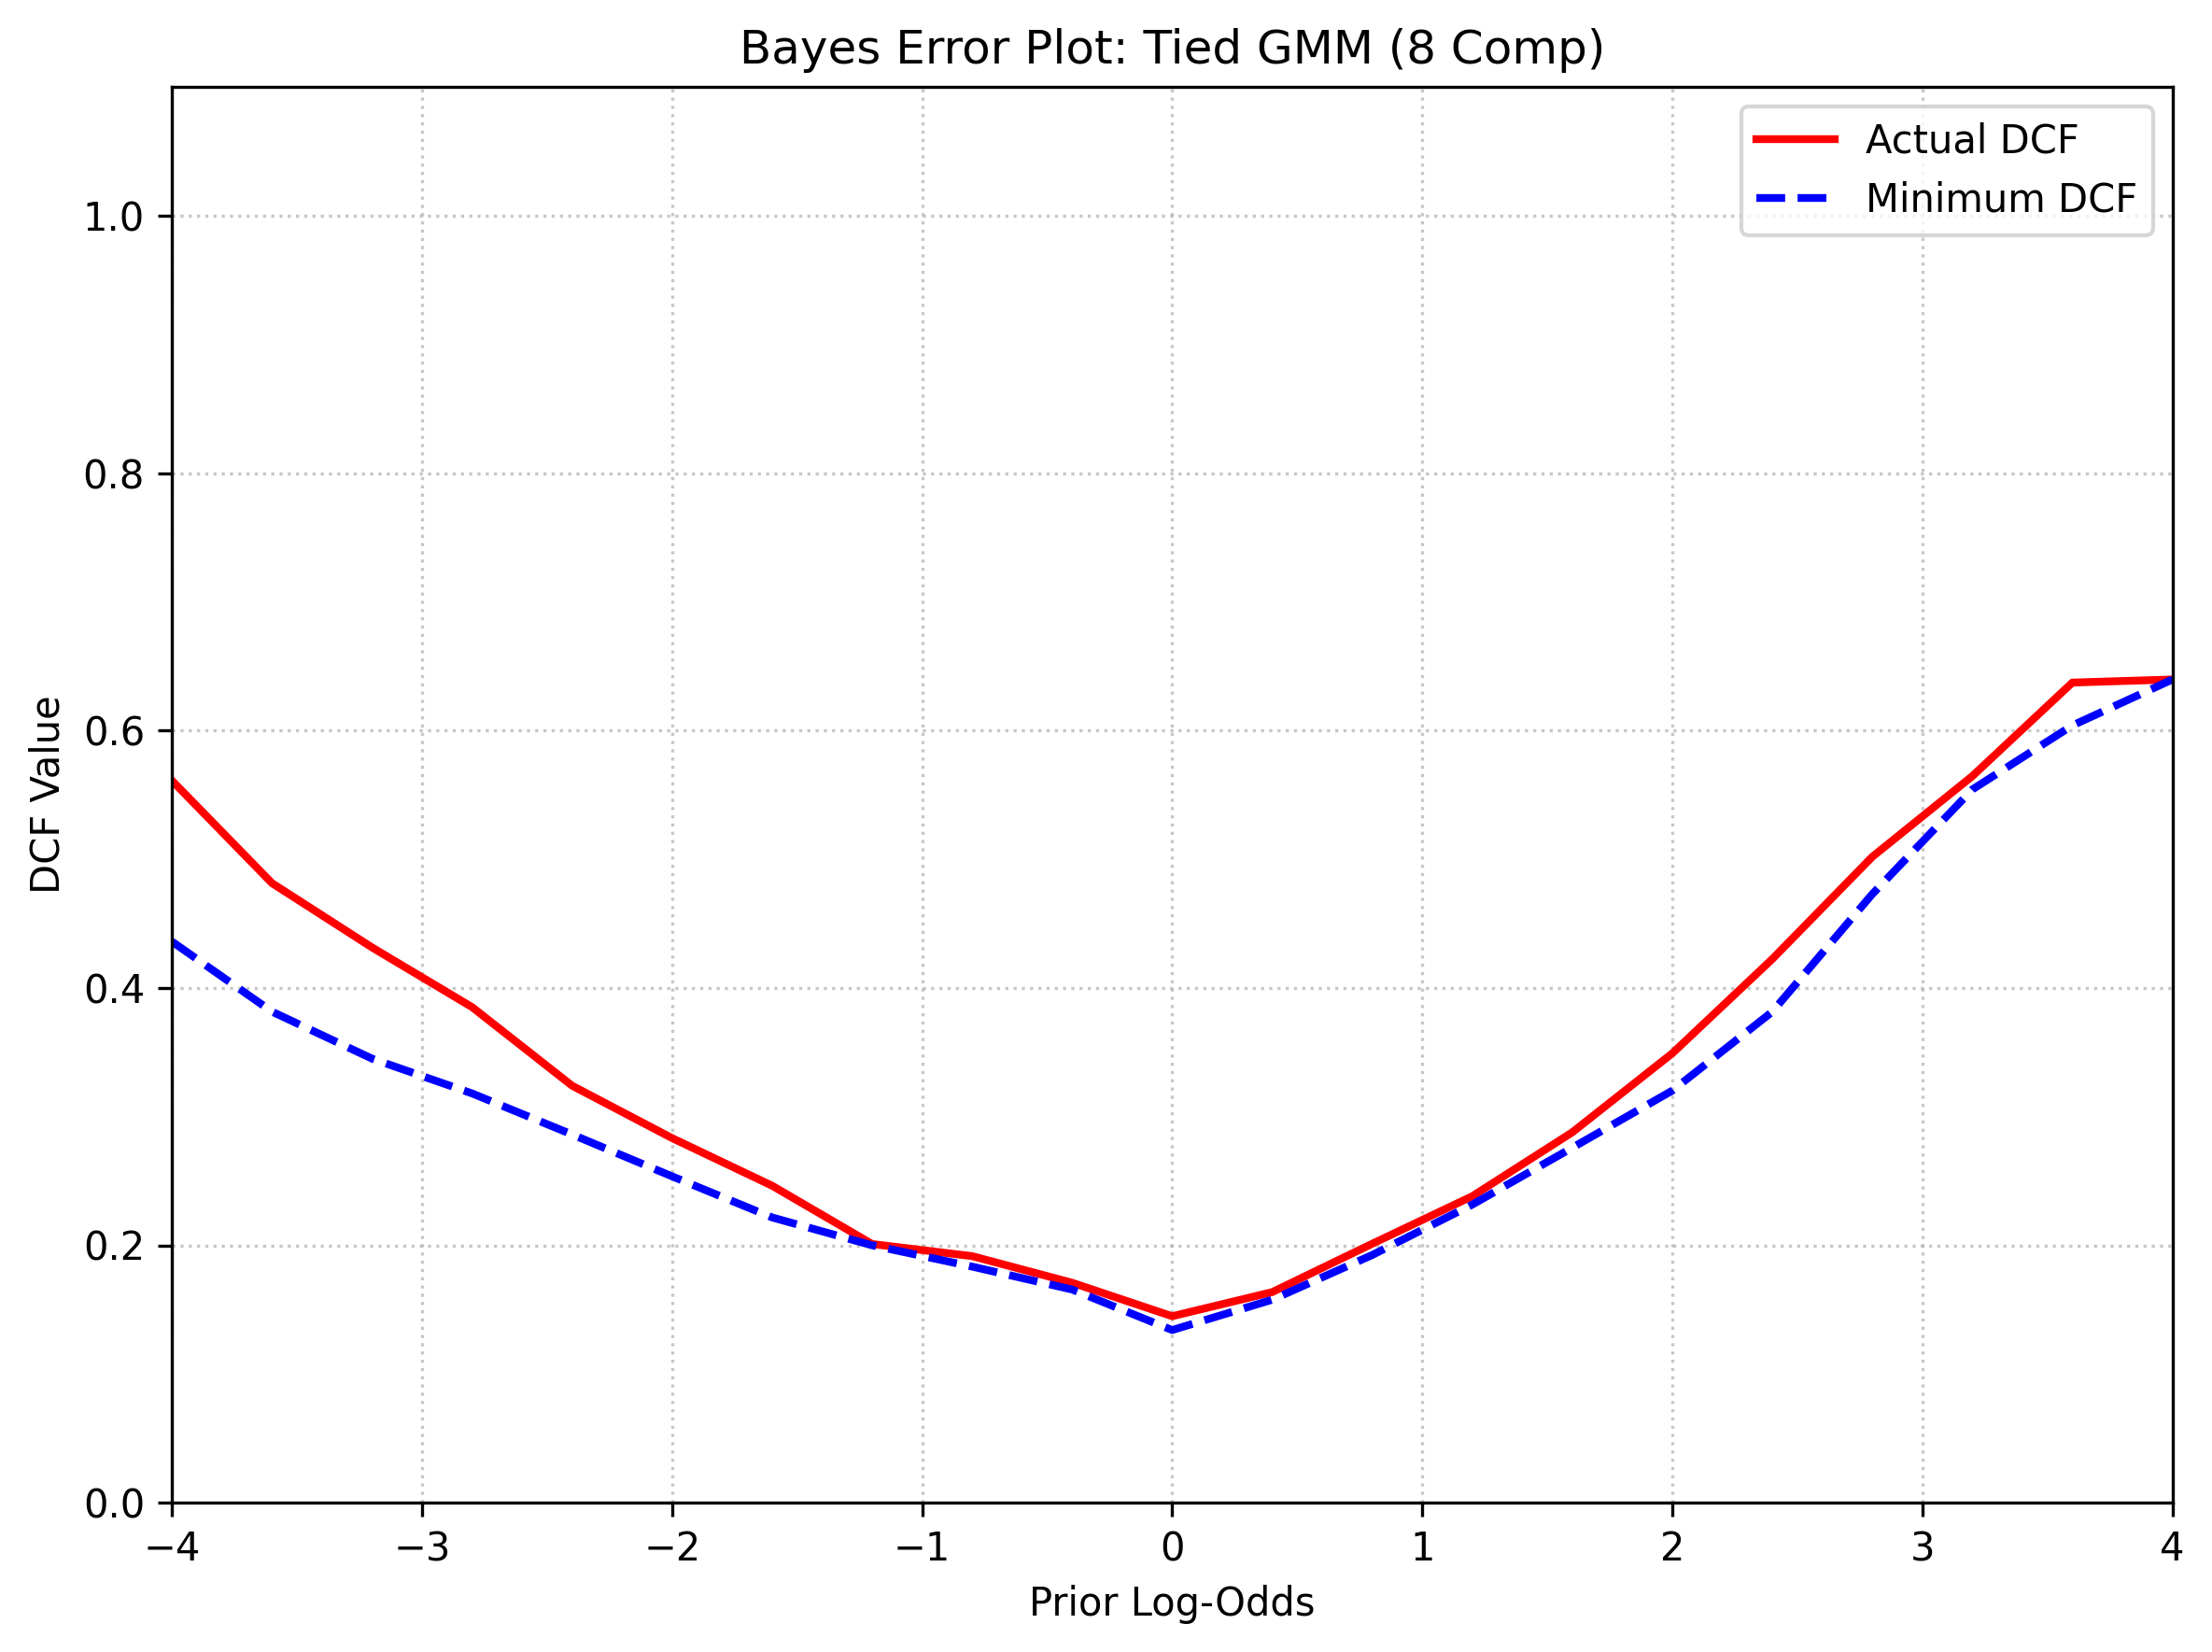
\includegraphics[width=0.75\textwidth]{bayes_error_tied_8comp.png}
    \caption{Bayes Error plot for the Tied Covariance GMM with 8 components. The overall error is visibly higher, and the calibration gap widens slightly at the extremes.}
    \label{fig:bayes_tied_8}
\end{figure}

\section{Analysis and theoretical considerations}

\subsection*{Question: What do you observe?}

Across all three plots, we observe the characteristic "V" shape or "trumpet" shape of the error curves, where the absolute cost peaks near the center (log-odds $= 0$, corresponding to a uniform prior) and naturally tapers off at the extreme ends of the spectrum. 

Most importantly, we observe that the overall profile of the GMM curves is situated extremely low on the y-axis compared to the plots from the Logistic Regression and SVM laboratories. The Diagonal 16-component model (Figure \ref{fig:bayes_diag_16}) maintains a minimum DCF well below $0.1$ for nearly the entire operational range, visually confirming its absolute dominance over the discriminative models.

\subsection*{Question: In terms of minimum DCF, are the results consistent, preserving the relative ranking of the systems?}

Yes, the results are perfectly consistent and strictly preserve the relative ranking of the systems across the entire log-odds spectrum. 

If we overlay the blue Minimum DCF curves from the three plots, the Diagonal 16-component model consistently traces the lowest path, followed very closely by the Full 8-component model. The Tied 8-component model's blue curve is visibly elevated above the others at all operating points (log-odds from $-4$ to $+4$). 

\textbf{Theoretical explanation:} Minimum DCF measures purely the ranking capability of the model (its ability to sort samples from most likely "Genuine" to most likely "Impostor"). Because the Diagonal GMM with 16 components successfully maps the true, uncorrelated variance of the dataset without suffering from parameter estimation noise, it inherently computes a superior geometric boundary. This superiority in class separation holds universally, regardless of the classification threshold dictated by the application's prior.

\subsection*{Question: What about actual DCF? Are there models that are well calibrated for most of the operating point range?}

Yes, the \textbf{Diagonal 16-component} (Figure \ref{fig:bayes_diag_16}) and \textbf{Full 8-component} (Figure \ref{fig:bayes_full_8}) GMMs are exceptionally well-calibrated for almost the entire operating point range. The red Actual DCF curves tightly hug the blue Minimum DCF curves from approximately $-3$ to $+3$ log-odds.

\textbf{Theoretical explanation:} GMMs are generative models, which they are optimized using Expectation-Maximization to directly estimate the true probability densities $f_{X|C}(x|c)$. As a result, the scores they produce are mathematically valid Log-Likelihood Ratios. Unlike the raw geometric distances output by an SVM (which caused massive calibration gaps), the GMM's LLRs natively align with the theoretical Bayes threshold ($t = -\log \frac{\pi_T}{1-\pi_T}$). This allows the models to execute highly optimal decisions out-of-the-box without explicit score recalibration.

\subsection*{Question: Are there models that show significant miscalibration?}

While none of the GMMs show the catastrophic miscalibration observed in the discriminative SVM models, the \textbf{Tied 8-component GMM} (Figure \ref{fig:bayes_tied_8}) does exhibit noticeable miscalibration (a visible vertical gap between the red and blue curves) at the extreme ends of the log-odds spectrum (e.g., beyond $+3$ and below $-3$). 

\textbf{Theoretical explanation:} Miscalibration at extreme operating points implies that the model's LLRs in the "tails" of the distribution are slightly inaccurate. By forcing a shared covariance matrix (Tied), the model fails to accurately describe the varying geometric spread of the two classes. This structural rigidity causes the estimated density tails to diverge from the true data distribution. When the application features an extreme prior (e.g., $\pi_T = 0.99$ or log-odds $\approx 4$), the decision threshold shifts deep into these poorly estimated tails, causing the empirical decisions (Actual DCF) to diverge from the optimal ranking potential (Minimum DCF).

\subsection*{Question: Are there models that are harmful for some applications?}

A model is considered mathematically "harmful" for a specific application if its Actual DCF exceeds $1.0$. An actDCF $> 1.0$ means the classifier is performing worse than a "dummy" system that simply predicts the most frequent class blindly based on the prior probability.

Looking at the plots, there are no models that are harmful for all applications, but the \textbf{Tied 8-component GMM} (Figure \ref{fig:bayes_tied_8}) becomes slightly bad at the extreme right edge of the spectrum (log-odds $\approx 4.0$), where the actuald DCF hits a value of $\approx 0.65$. 

\textbf{Theoretical explanation:} At extreme log-odds, the system is overwhelmingly biased toward one class. To contradict this heavy prior and predict the rare class, the classifier must produce an extreme LLR. If the model's density estimation is structurally flawed (as is the case with the Tied covariance assumption on our dataset), it may produce overconfident, erroneous LLRs that cross this extreme threshold. When the model consistently makes incorrect predictions that contradict a heavily favored prior, it accumulates a cost higher than simply predicting the default class, rendering the active deployment of the model actively harmful to the system's error rate.